\begin{frame}{Integrative Modelling Platform}
    Now we already know what is IMP. It is computationally expensive and time consuming due Markov Chain Monte Carlo (MCMC) sampling. \\
    \bigskip
    \pause
    We wish to replace the computationally expensive sampling techniques to paradigms used in DREAM: \\
    \begin{itemize}
        \item Orientate the structures of subunits based on experimental evidence which is similar to substruture computation in DREAM
        \item Register the subunits in one shot while respecting the experimental evidence. (an enhancement of DREAM's registration)
    \end{itemize}
\end{frame}

\begin{frame}{How will this happen ?}
    \begin{itemize}
        \item Our substructures in this case are different kinds of proteins. \\
        \item We have cross-links data available these proteins. \\
    \end{itemize}

    Given this information, we need to do one shot registration of these proteins to model the structure of complex.

\end{frame}

\begin{frame}{}
    \begin{figure}
        \centering
        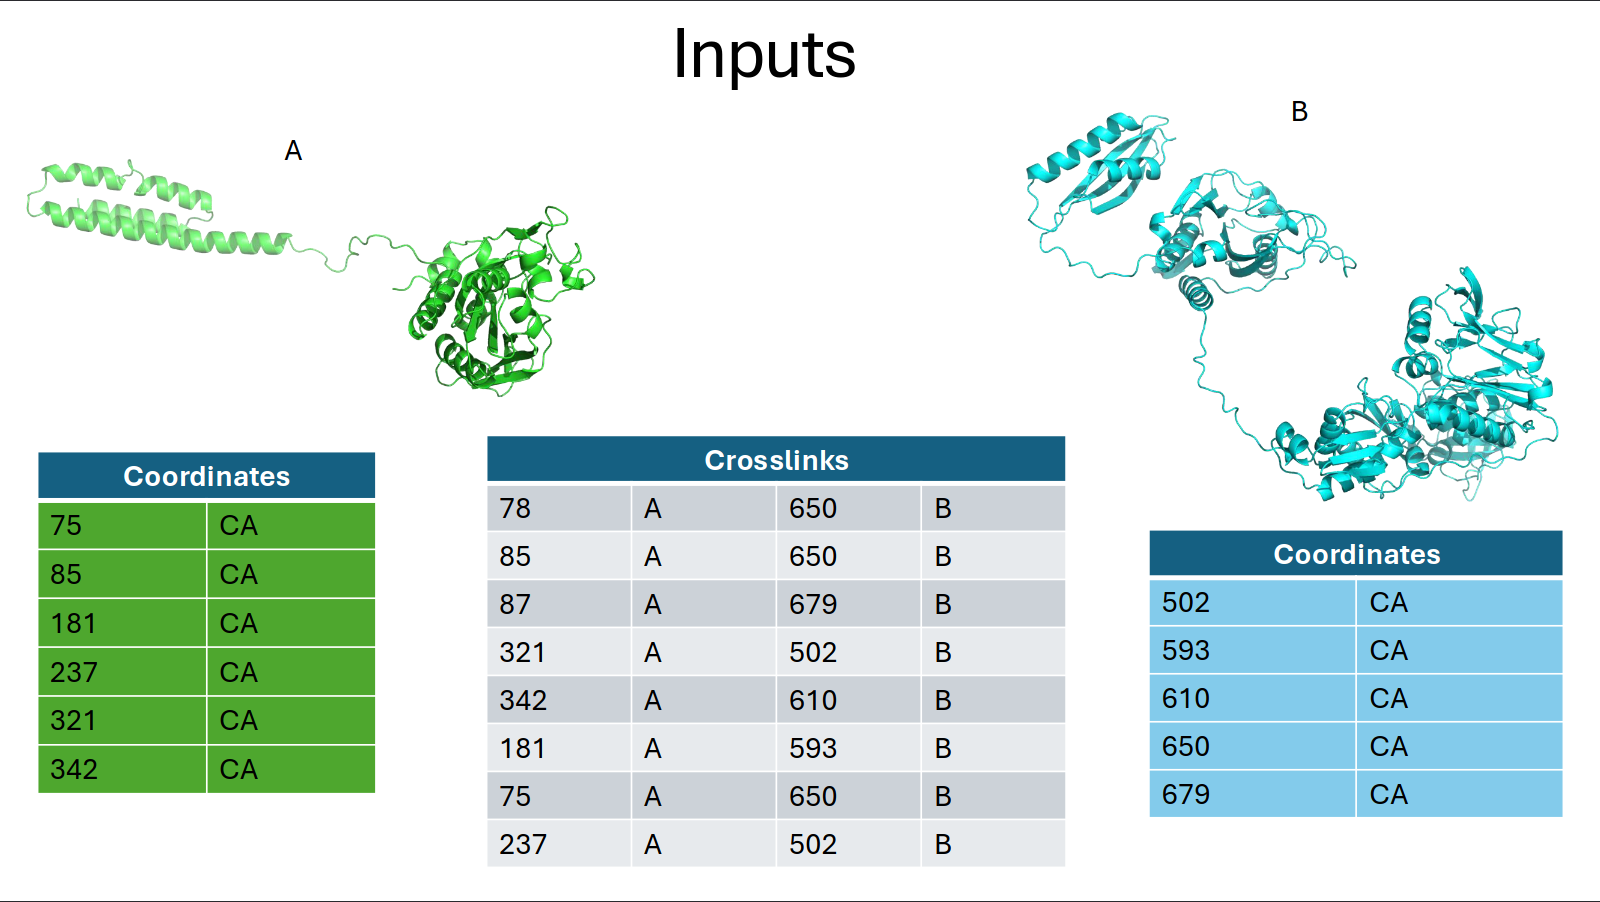
\includegraphics[width=1\textwidth]{images/local.png}
        \caption{Example of 2 proteins with cross-links data}
        \label{fig:my_label}
    \end{figure}
\end{frame}

\begin{frame}{Problem}
    \begin{figure}
        \centering
        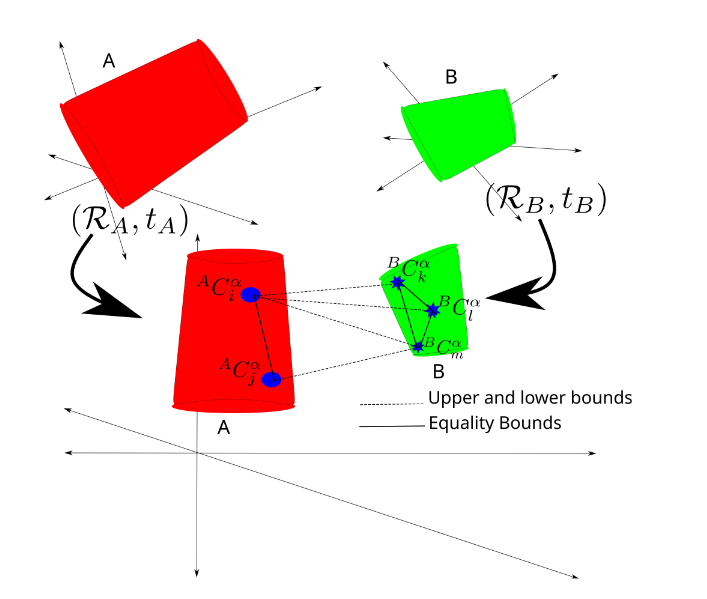
\includegraphics[width=0.7\textwidth]{images/toy1.png}
        \caption{Consider A,B as proteins and the lines as cross-links}
        \label{fig:my_label}
    \end{figure}
\end{frame}

\begin{frame}{Solution}
    \begin{figure}
        \centering
        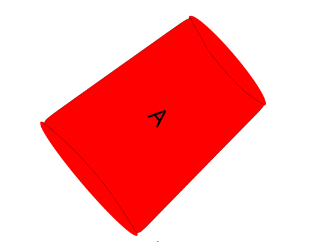
\includegraphics[width=0.3\textwidth]{images/A.png}
        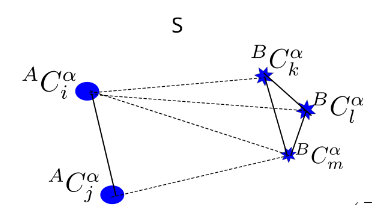
\includegraphics[width=0.3\textwidth]{images/S.png}
        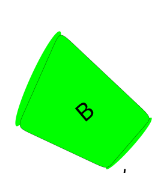
\includegraphics[width=0.3\textwidth]{images/B.png}
        \label{fig:my_label}
    \end{figure}
    Consider S as hypothetical framework. 
    \pause
    Then we can do one shot registration of A,S and B
\end{frame}

\begin{frame}{Solution}
    \begin{figure}
        \centering
        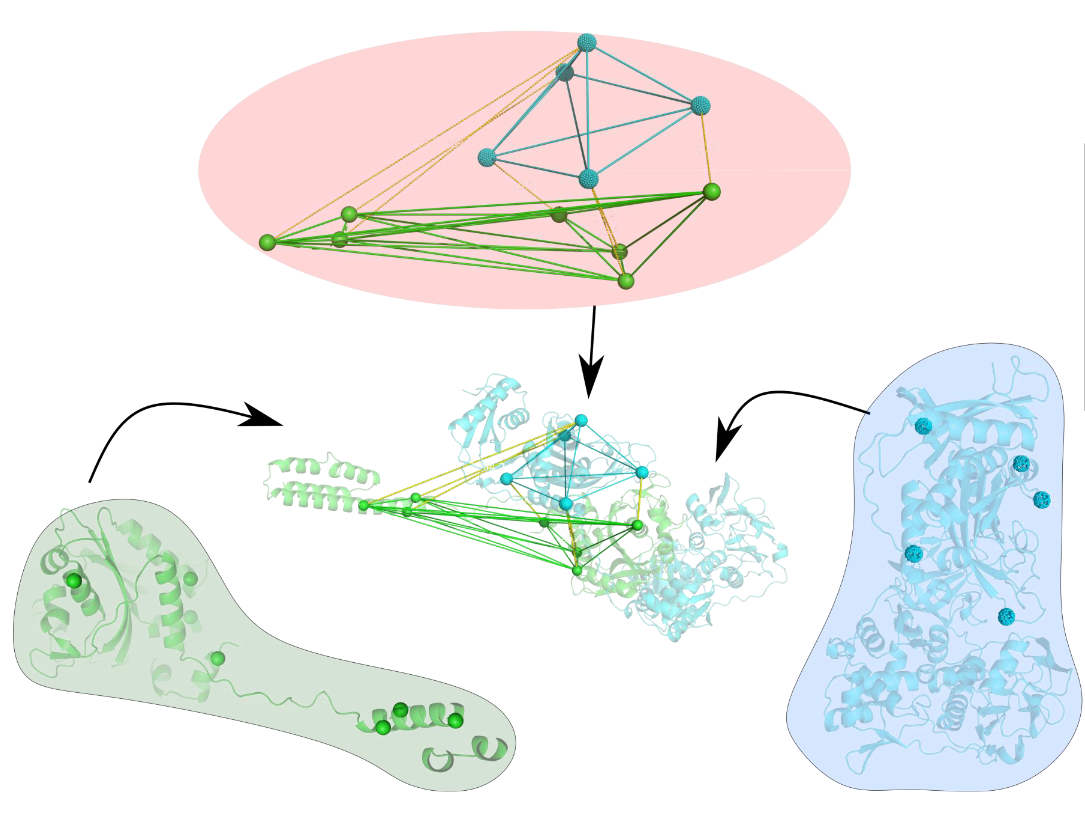
\includegraphics[width=0.7\textwidth]{images/final.png}
        \caption{One shot registration}
        \label{fig:my_label}
    \end{figure}
\end{frame}

\begin{frame}{Some Observations}
    1. In the hypothetical framework, we have all pairs of distances between C-alpha atoms in each protein. \\
    \pause
    2. For registering n proteins, only 1 hypothetical fragment is needed. So registration of $n+1$ proteins is done. \\
\end{frame}